\documentclass[12pt]{article}

%\usepackage[showframe]{geometry}
\usepackage{enumerate, amsmath, wasysym, float, graphicx, titling}

\setlength{\droptitle}{-5em}
\author{Carl Denton}
\title{Numerically Solving Burgers and KPZ Equations}
\date{\vspace{-6ex}}
\begin{document}
\maketitle

\section{Introduction}

The Burgers equation is a nonlinear PDE that arises in a variety of contexts (including as a one-dimensional equivalent of the incompressible Navier-Stokes equations). In this homework we solve the Burgers equation as well as the related Kardar-Parisi-Zhang equation (a stochastic PDE describing phenomena such as interface growth).

\section{Problem}

The Burgers equation is given by
\[\partial_t u + u\partial_x u = \nu \partial_{xx} u\]
and the KPZ equation is given by
\[\partial_t h = \frac{\lambda}{2}\left( \nabla h\right)^2 + \nu \nabla^2h + r\xi\]
where $\xi$ is unit-variance Gaussian white noise and $r$ is a scaling factor. We saw in class that the two equations are equivalent (up to stochasticity) by the substitution $u = -\partial_x h$. The aim of this assignment is to solve these equations numerically.

\section{Methods}
We primarily use finite difference methods to solve the equations. That is, for the Burgers equation, we have
\[u_j^{n+1} = u_j^n - \frac{u_j^n\Delta t}{2\Delta x}\left(u_{j+1}^n - u_{j-1}^n\right) + \frac{\nu \Delta t}{\Delta x^2} \left(u_{j+1}^n - 2u_j^n+u_{j-1}^n\right)\]
To check our solutions we perform standard convergence tests diffusive scaling and check the order of the rror. 
For the KPZ equation we have
\[h_j^{n+1} = h_j^n + \frac{\lambda \Delta t}{8\Delta x^2} \left(h_{j+1}^n - h_{j-1}^n\right)^2 + \frac{\nu \Delta t}{\Delta x^2}\left(h_{j+1}^n - 2h_j^n + h_{j-1}^n\right) + \xi_j^n\]
in one dimension, and 
\begin{align*}
 h_{j, k}^{n+1} &= h_{j, k}^n + \frac{\lambda \Delta t}{8 \Delta x^2}\left(h_{j+1, k}^n - h_{j-1,k}^n + h_{j, k+1}^n - h_{j, k-1}^n \right)^2 \\
&+ \frac{\nu\Delta t}{\Delta x^2} \left(h_{j+1, k}^n + h_{j-1, k}^n + h_{j, k+1}^n + h_{j, k-1}^n - 4h_{j, k}^n \right) + \xi_{j, k}^n
\end{align*}
in two dimensions.
To validate, we check scaling laws for the numerical solutions.

\section{Experiments}

\subsection{Burgers Equation}

\subsubsection{Simulation}

The results of the simulation for $N = 100$ grid points, $\text{Re} = \frac{|u_j^n|L}{\nu} = |u_j^n| \times 10^2$, with Gaussian initial conditions, look as follows (at $n\Delta t = 0, 25, 50$):
\begin{figure}[H]
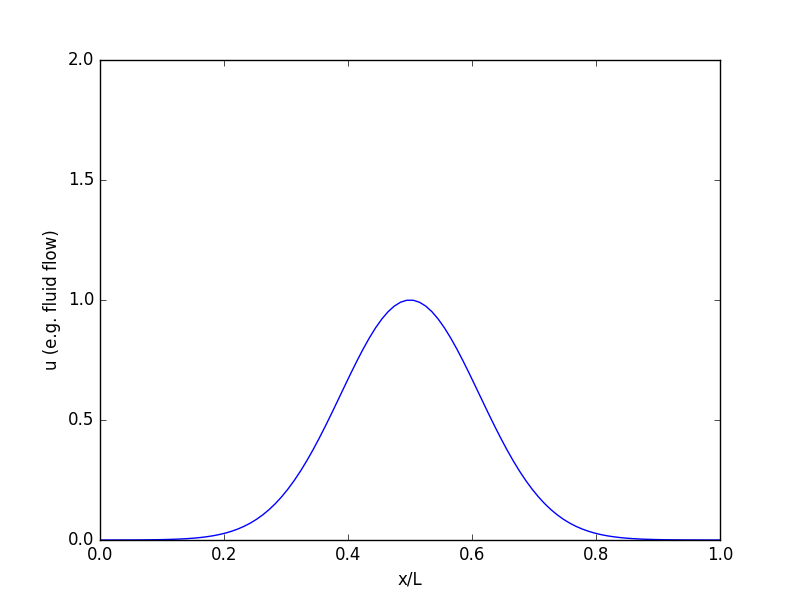
\includegraphics[width=.32\hsize]{burgers0.png} 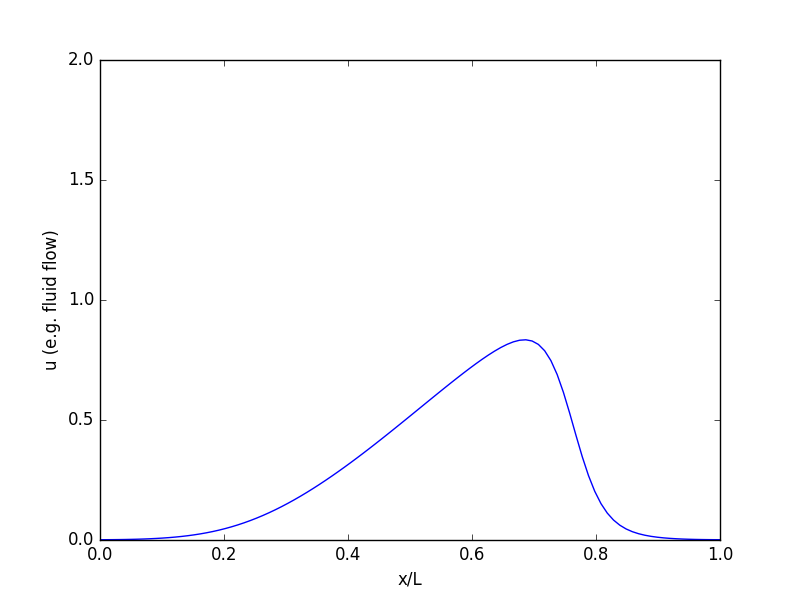
\includegraphics[width=.32\hsize]{burgers250.png} 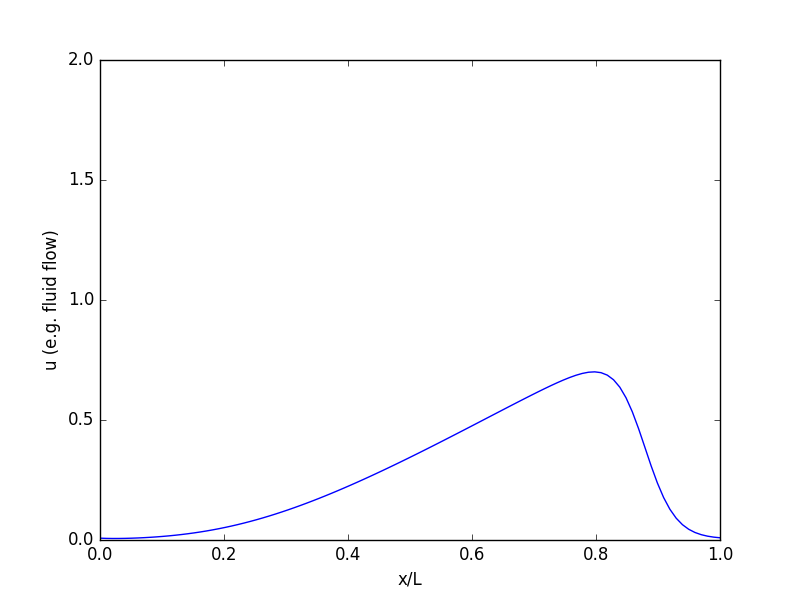
\includegraphics[width=.32\hsize]{burgers500.png}
\end{figure}
\noindent For the alternative choice of parameters such that $\text{Re} = \frac{|u_j^n|L}{\nu} =  |u_j^n|\times 10^{-2}$, we get the following (now with $n\Delta t = 0, .025, .05$):
\begin{figure}[H]
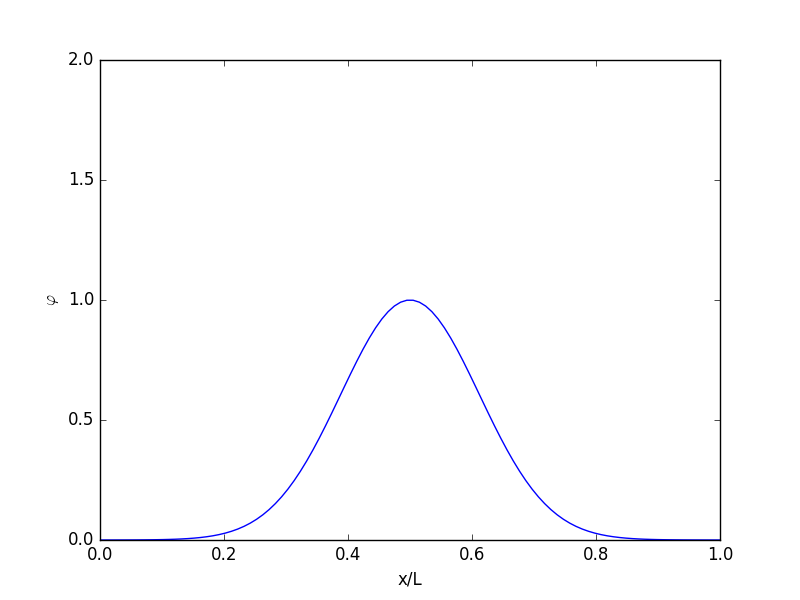
\includegraphics[width=.32\hsize]{burgers2-0.png} 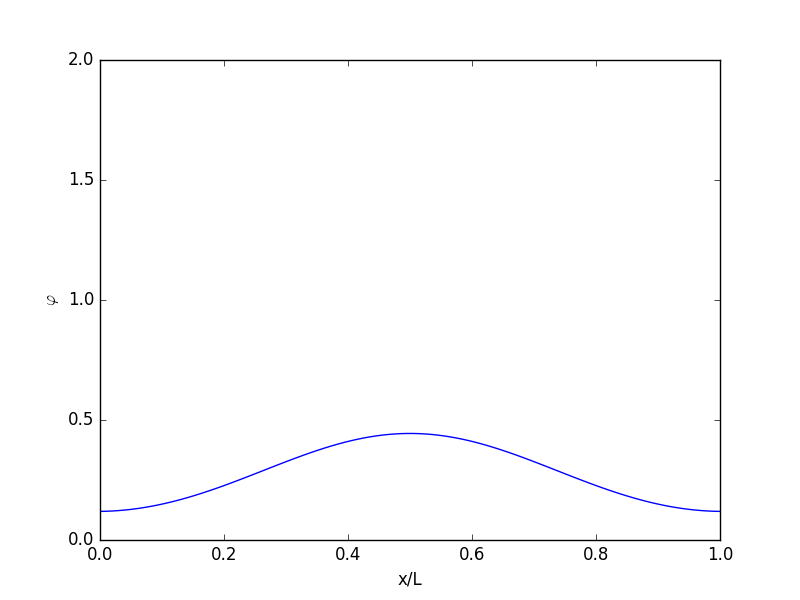
\includegraphics[width=.32\hsize]{burgers2-2500.png} 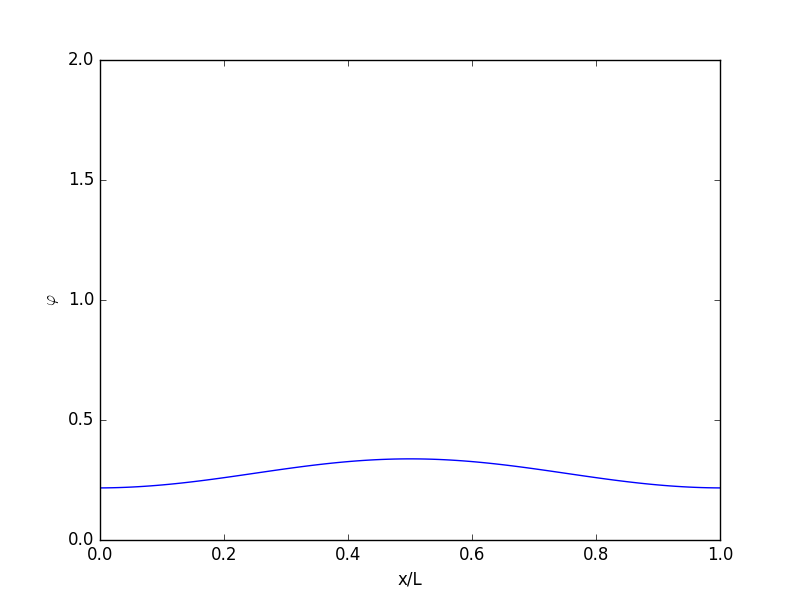
\includegraphics[width=.32\hsize]{burgers2-5000.png}
\end{figure}
\noindent Thus we get far more diffusive solutions at low Reynolds numbers, as we might expect.

\subsubsection{Validation}

We check the validity of the method by testing grid convergence with diffusive scaling as usual, with the following results:
\begin{figure}[H]
\center{
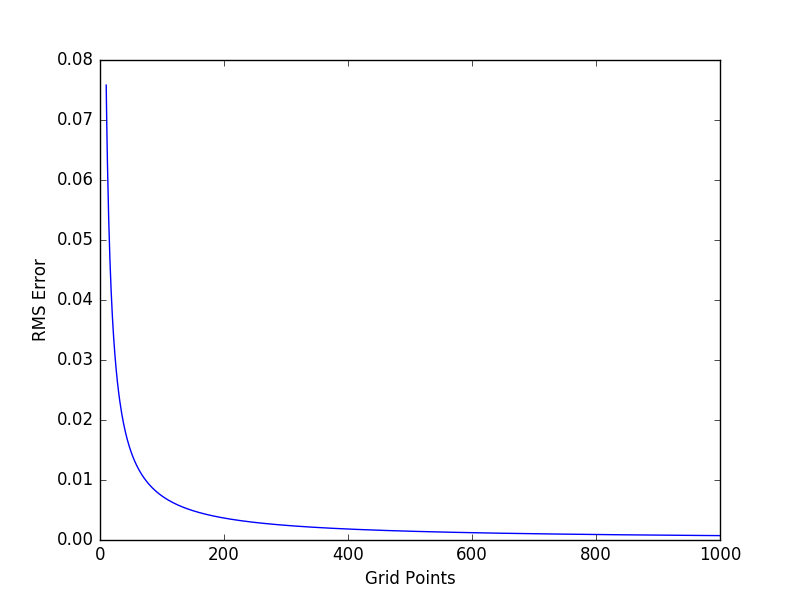
\includegraphics[width = .75\hsize]{burgers-convergence.png}
}
\end{figure} 
\noindent We also check the order of our method by computing
\[\frac{\varphi_{\Delta x} - \varphi_{\Delta x/2}}{\varphi_{\Delta x/2} - \varphi_{\Delta x/4}} = \frac{\varepsilon\left(\Delta x^n - \Delta x^n/2^n\right)}{\varepsilon\left(\Delta x^n/2^n - \Delta x^n/4^n\right)} = 2^n\]
where $\varphi_{\Delta x}$ is the numerical solution with spatial interval $\Delta x$, and we have assumed that 
\[\varphi = \varphi_{\Delta x} + \varepsilon\Delta x^n\]
for exact solution $\varphi$. An identical computation can be used to find the order of the method in time. The results are as follows:
\begin{figure}[H]
\center{
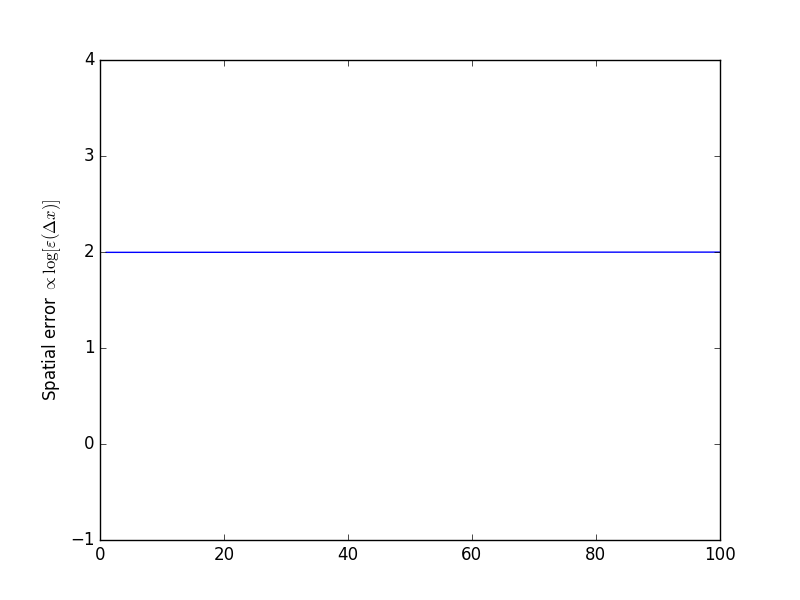
\includegraphics[width=.49\hsize]{space-order.png} 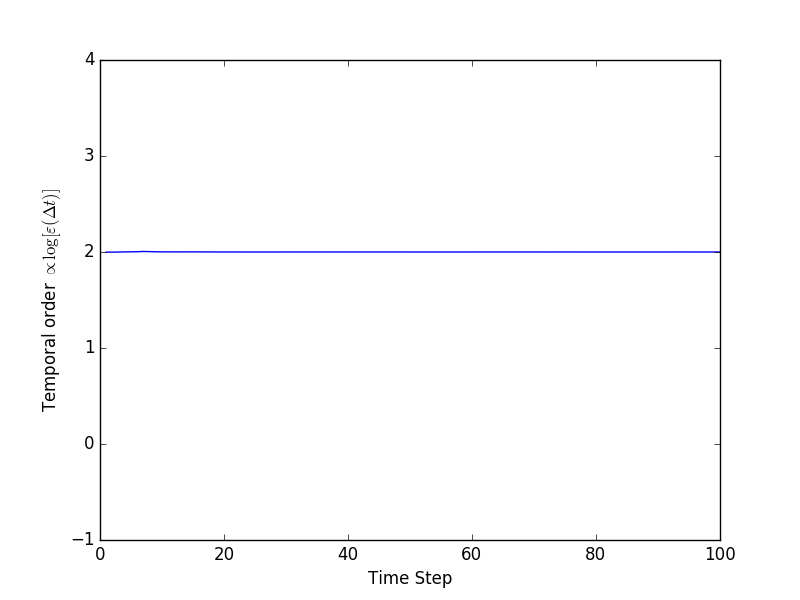
\includegraphics[width=.49\hsize]{time-order.png}
}
\end{figure}
That is, the method seems to be first-order in both space and time (I'm not sure I have a good explanation for this since it seems as though the method ought to be second order in space).

\subsection{KPZ Equation}

{\it One Dimension:}

With $\lambda \Delta t/\nu = 1\times 10^4$, the results of the 1-dimensional simulation are as follows (at time steps $t = 0, 25, 50$):
\begin{figure}[H]
\center{
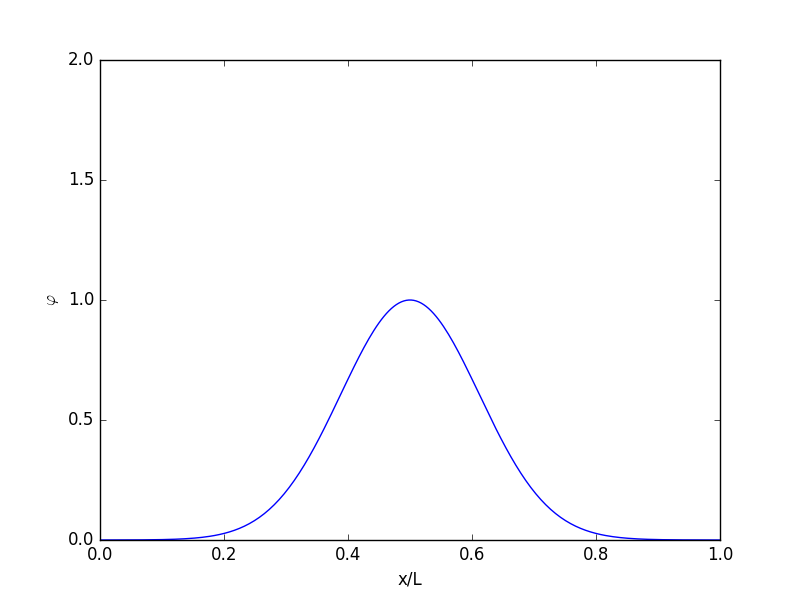
\includegraphics[width=.32\hsize]{kpz-0.png} 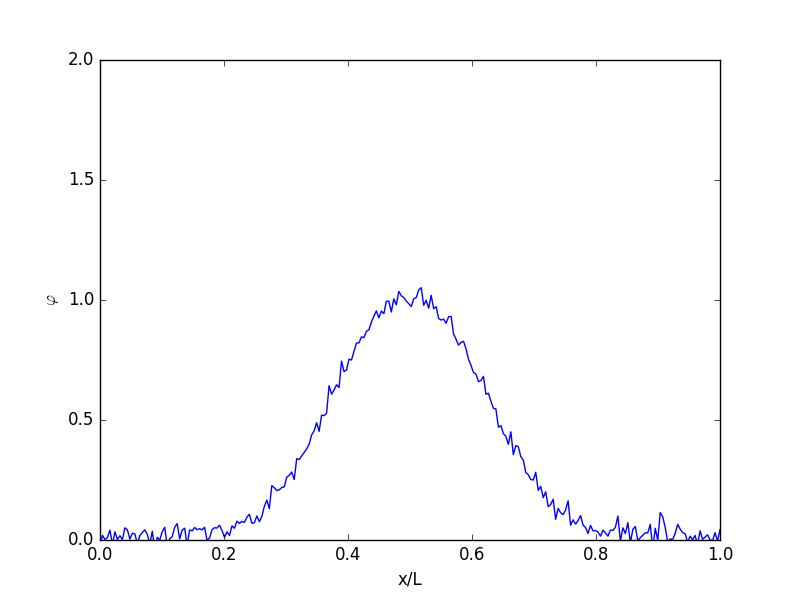
\includegraphics[width=.32\hsize]{kpz-500.png} 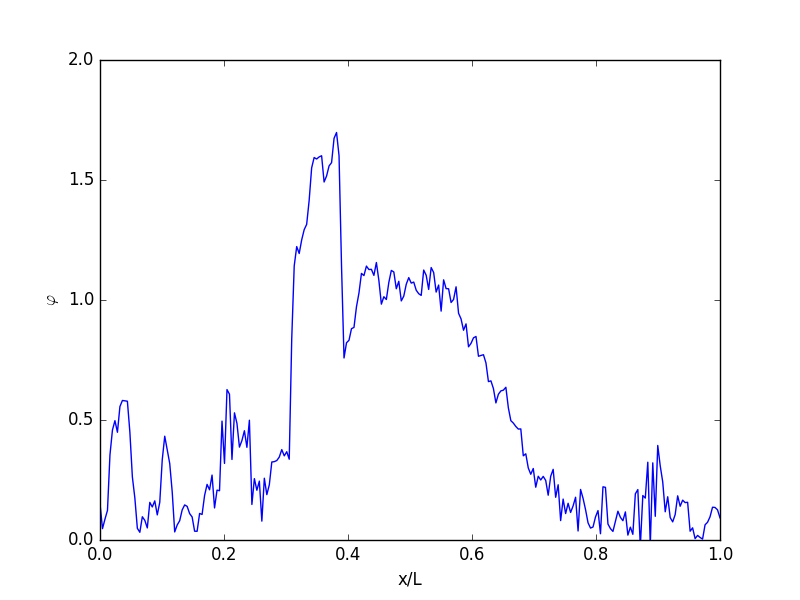
\includegraphics[width=.32\hsize]{kpz-1000.png} 
}
\end{figure}
\noindent On the other hand, $\lambda \Delta t/\nu = 1\times 10^3$ yields:
\begin{figure}[H]
\center{
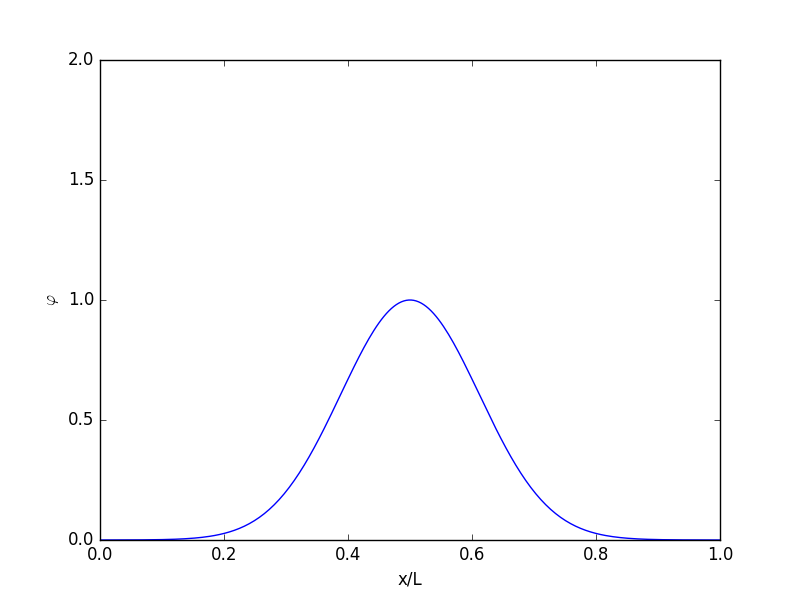
\includegraphics[width=.32\hsize]{kpz2-0.png} 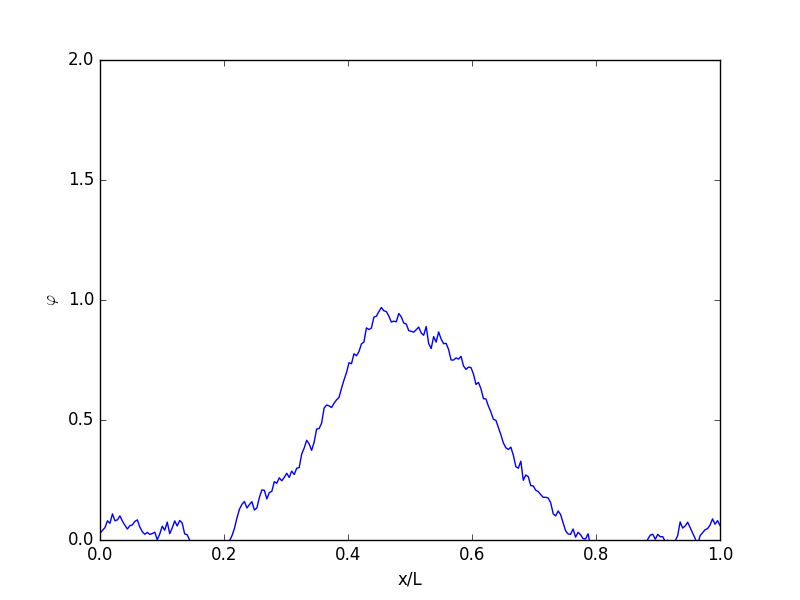
\includegraphics[width=.32\hsize]{kpz2-500.png} 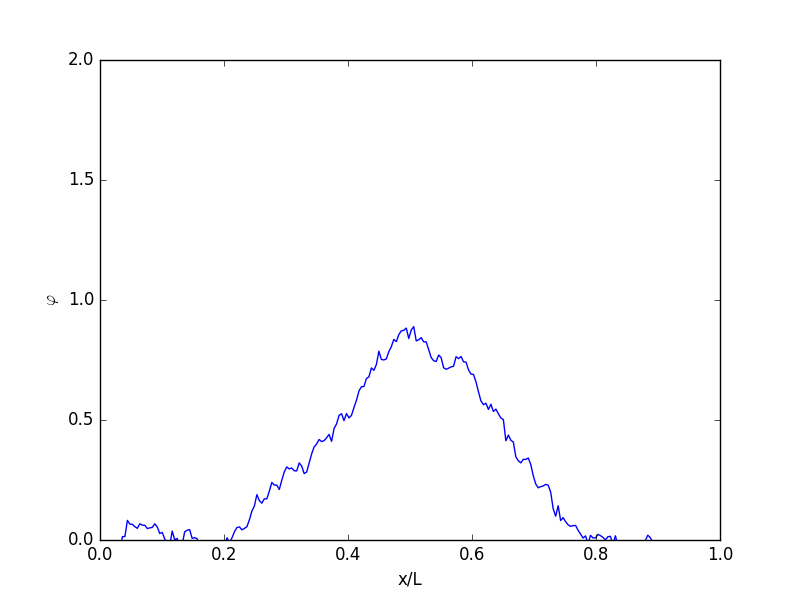
\includegraphics[width=.32\hsize]{kpz2-1000.png} 
}
\end{figure}
\noindent As expected, this solution is more diffusive. We also solve the equation for uniform initial conditions, which make the growth phenomena even more apparent ($\lambda \Delta t/\nu = 1$, $n\Delta t = 0, 2.5, 5.0, 50.0$):
\begin{figure}[H]
\center{
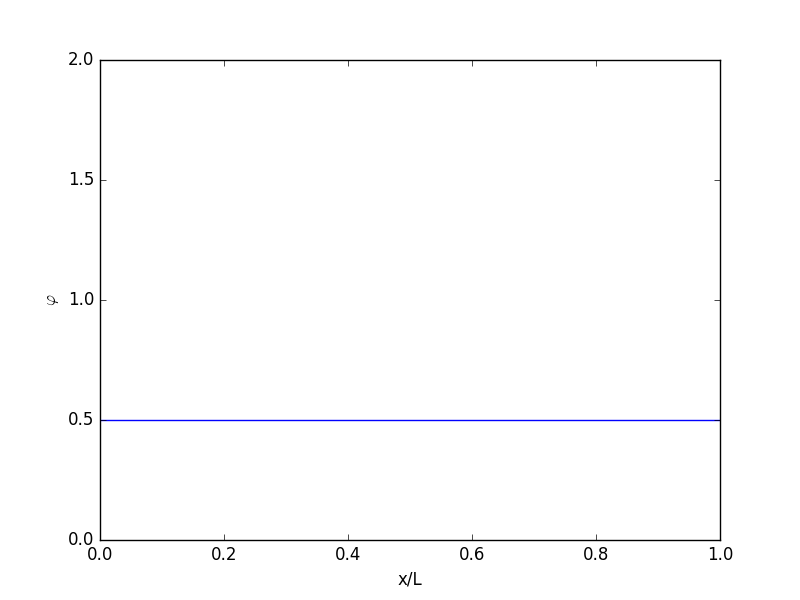
\includegraphics[width=.49\hsize]{kpz3-0.png} 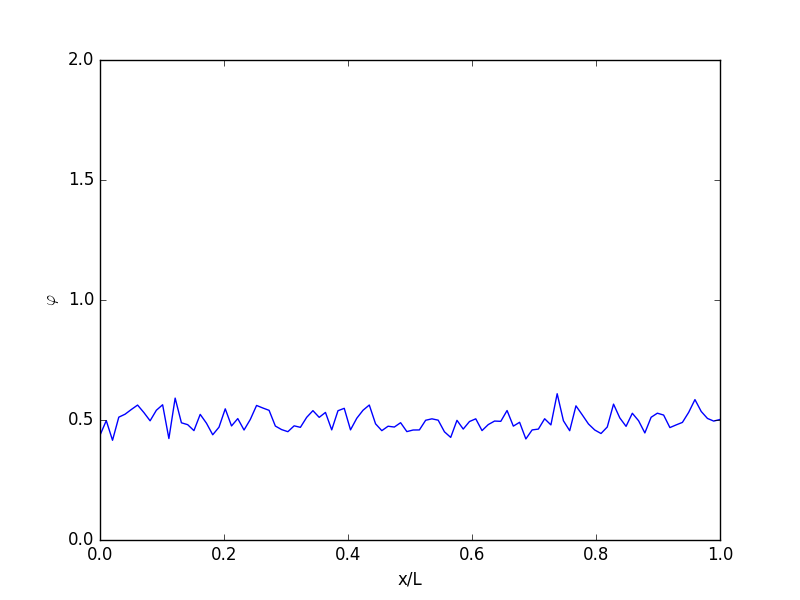
\includegraphics[width=.49\hsize]{kpz3-25.png} \\
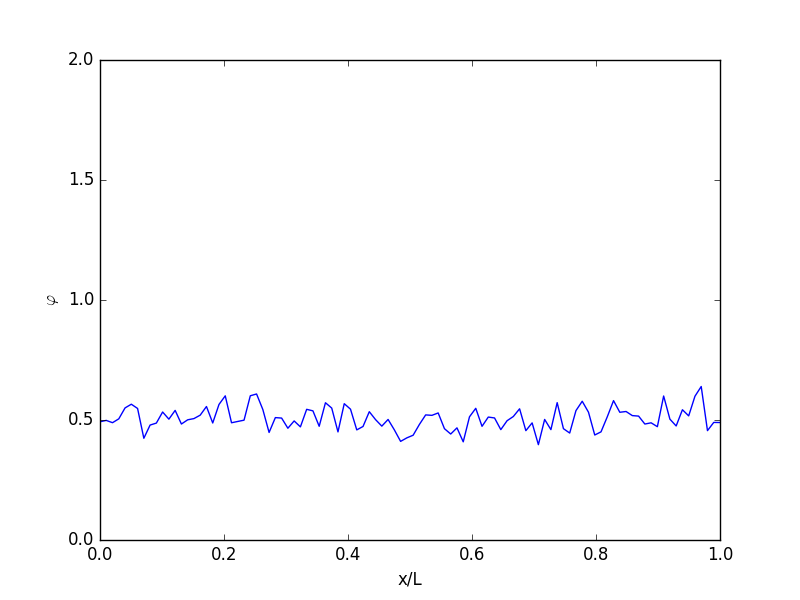
\includegraphics[width=.49\hsize]{kpz3-50.png}  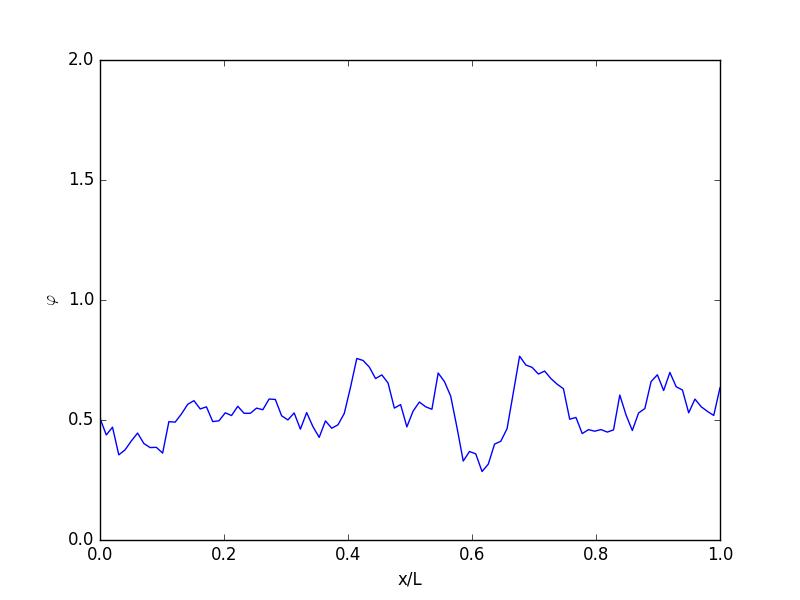
\includegraphics[width=.49\hsize]{kpz3-500.png} 
}
\end{figure}

\noindent {\it Two Dimensions:}

We perform similar experiments in two dimensions. With $N = 100^2$ total grid points and $\lambda \Delta t/\nu = .1$, we get (at time $n\Delta t = 0, 1.0, 2.0, 50.0$).
\begin{figure}[H]
\center{
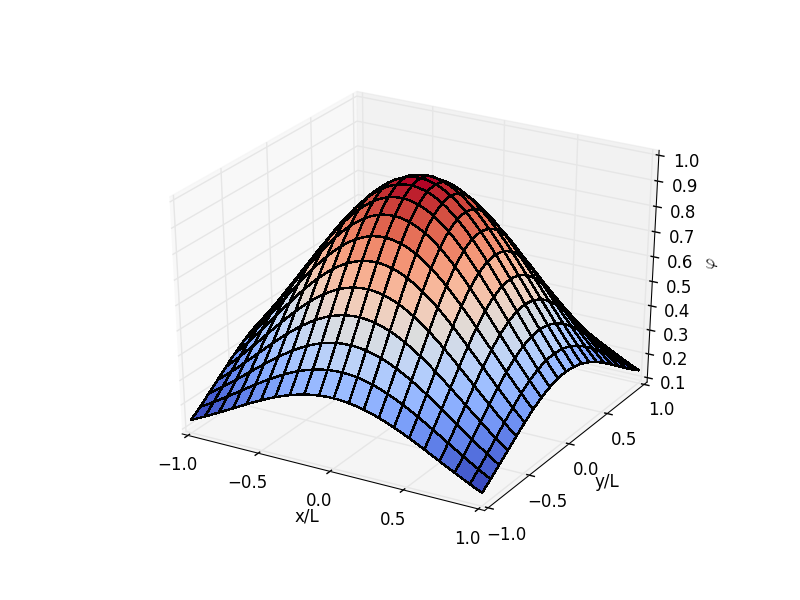
\includegraphics[width=.4\hsize]{kpz2D-0.png} 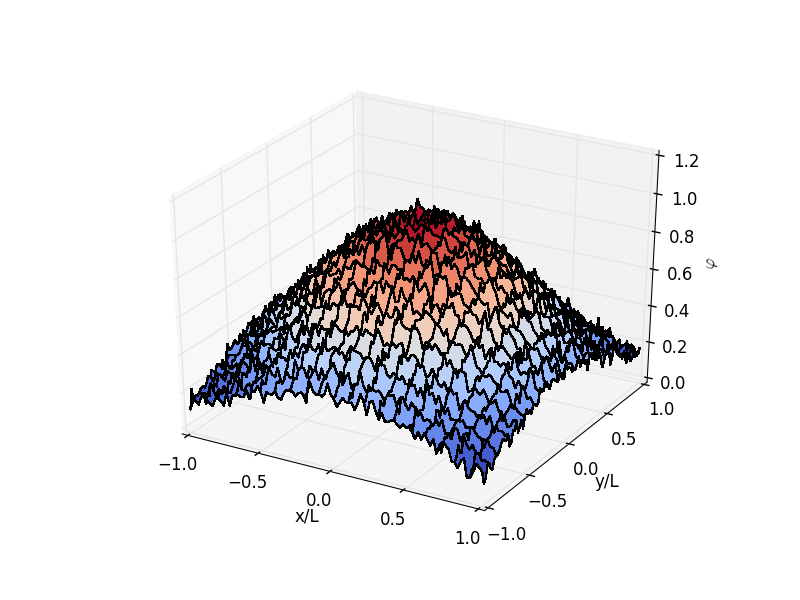
\includegraphics[width=.4\hsize]{kpz2D-10.png} \\
}
\end{figure}
\begin{figure}[H]
\center{
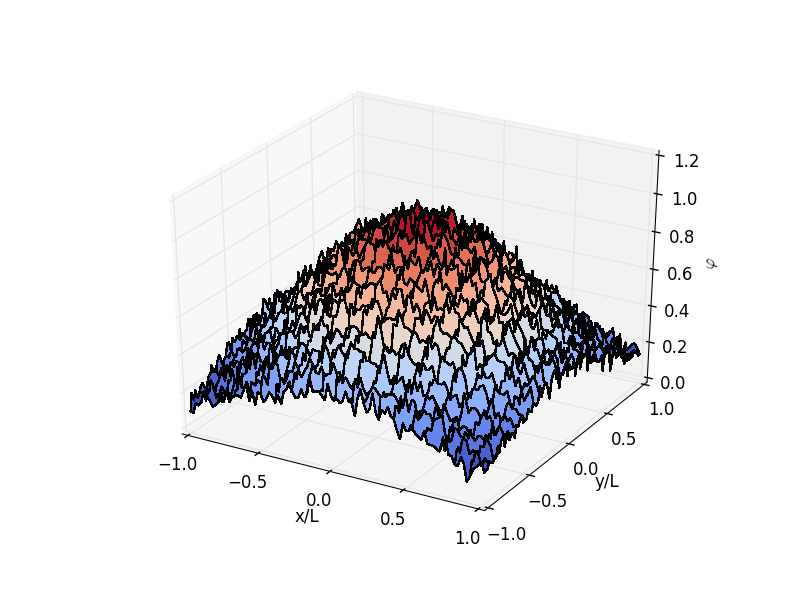
\includegraphics[width=.4\hsize]{kpz2D-20.png} 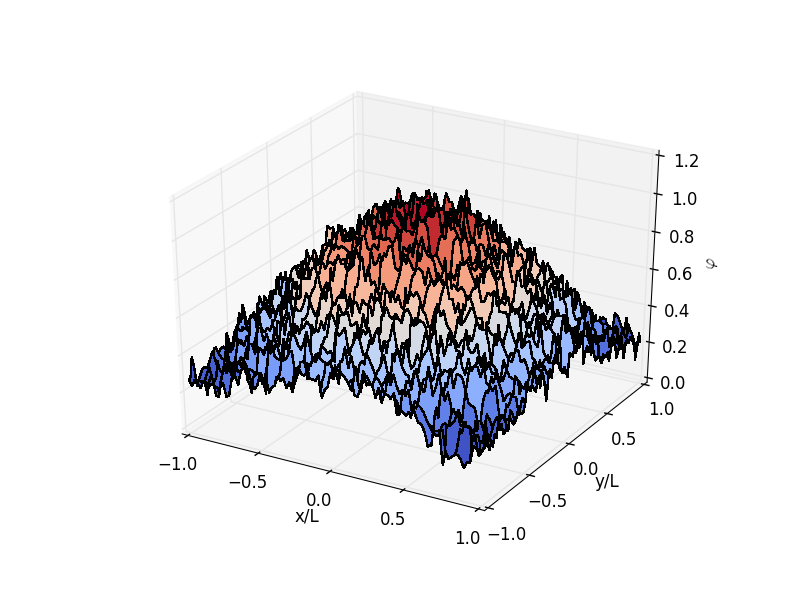
\includegraphics[width=.4\hsize]{kpz2D-500.png}
}
\end{figure}

We perform similar experiments in two dimensions. With $N = 100^2$ total grid points and $\lambda \Delta t/\nu = 1$, we get (at time $n\Delta t = 0, .5, 1.0, 1.5$).
\begin{figure}[H]
\center{
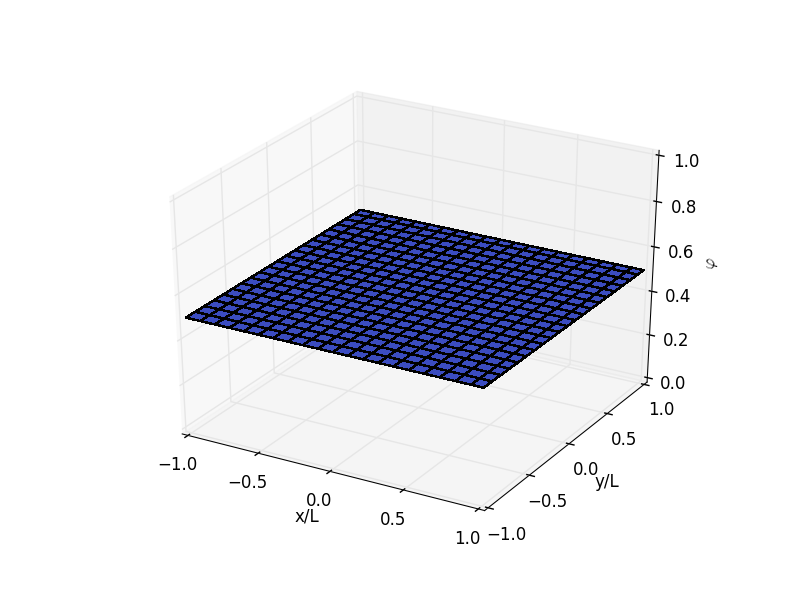
\includegraphics[width=.4\hsize]{kpz2D-2-0.png} 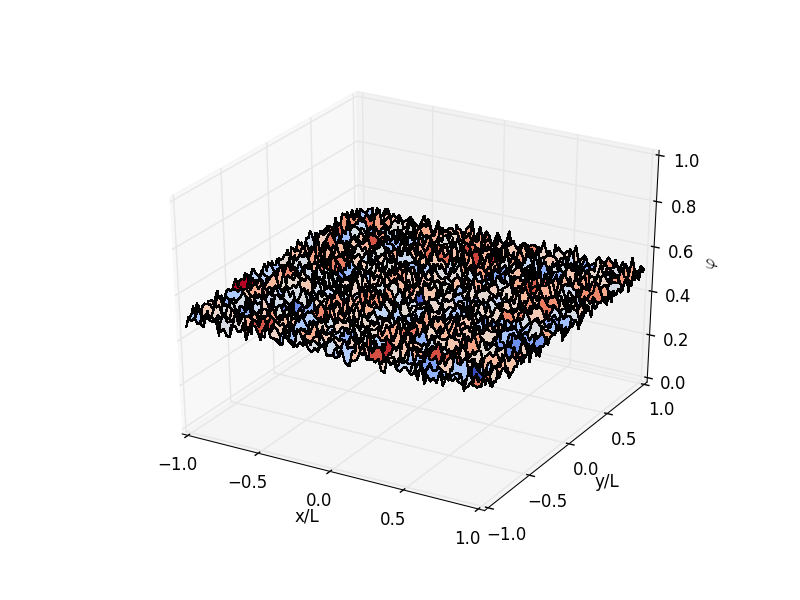
\includegraphics[width=.4\hsize]{kpz2D-2-5.png} \\
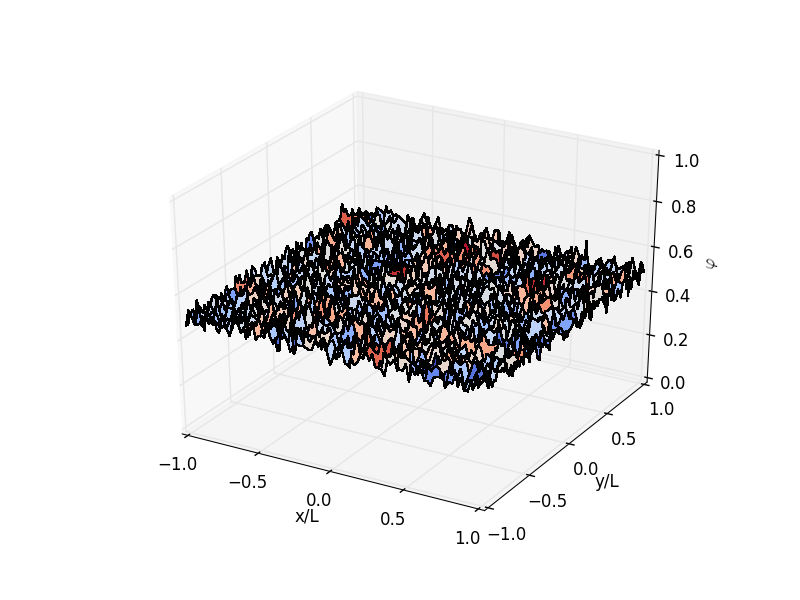
\includegraphics[width=.4\hsize]{kpz2D-2-10.png} 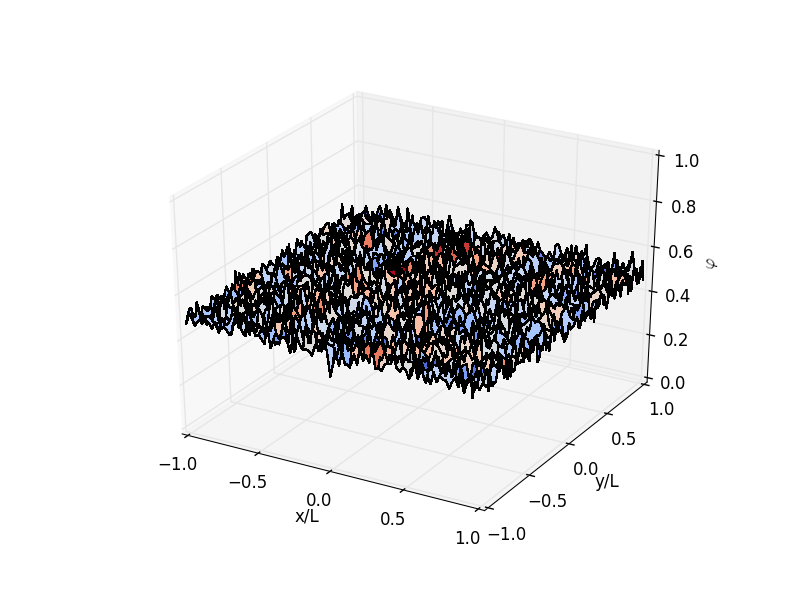
\includegraphics[width=.4\hsize]{kpz2D-2-15.png}
}
\end{figure}

\subsubsection{Validation}

We validate our solutions by checking the scaling laws seen in lecture. That is, for a solution of the KPZ equation, we expect that 
\[L^a f(t/L^z)\]
where 
\[f(x) = \begin{cases}x^b & \text{ if $x \ll 1$} \\ 1 & \text{ if $x \gg 1$} \end{cases}\]
and $a = 1/2, b = 1/3, z = a/b$ in the one dimensional case.
Plotting the variance against our prediction from the scaling laws, we get the following:
\begin{figure}[H]
\center{
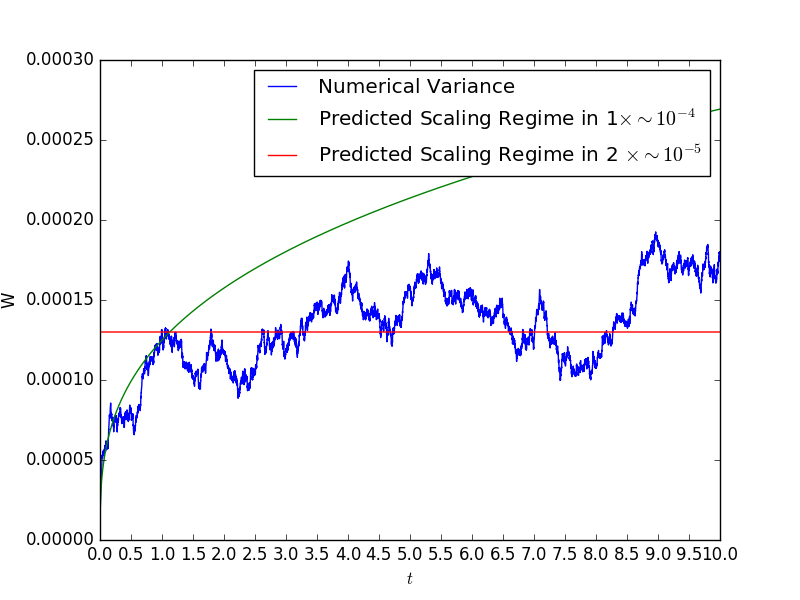
\includegraphics[width=.85\hsize]{kpz-scaling.png}
}
\end{figure}
\noindent Note that we had to scale the expected scaling by small constant factors for the scales to match--- this may be due to a difference in how noise was computed from the slides (we use arbitrarily scaled Gaussian noise). 
However, the essential features of the scaling can be seen clearly: the variance obeys a power law until $t$ becomes significantly large, at which point it becomes approximately constant.






\end{document}
